\documentclass[11pt,class=report,crop=false]{standalone}
\usepackage[screen]{../mathgame}
%\usepackage{xinttools}

\begin{document}


%====================================================================
\chapitre{Triangulation}
%====================================================================

%
%\insertvideo{yUgpElITYTg}{partie 5.1. Bits classiques}
%
%\insertvideo{iET0snUXj0k}{partie 5.2. Portes logiques}
%
%\insertvideo{JKmC2u5kvKg}{partie 5.3. Algorithme et complexité}



\objectifs{Nous découpons le plan en objets simples : des triangles.}


%%%%%%%%%%%%%%%%%%%%%%%%%%%%%%%%%%%%%%%%%%%%%%%%%%%%%%%%%%%%%%%%%%%%%
\section{Graphes}

%--------------------------------------------------------------------
\subsection{Vocabulaire}

\begin{itemize}
	\item Un \defi{graphe}\index{graphe} est un ensemble de \defi{sommets} et d'\defi{arêtes}. Une arête commence à un sommet et se termine à un sommet, on dit alors que les sommets sont \defi{adjacents}.	
	
\myfigure{0.6}{
	\tikzinput{graphe-01}
}	

	\item Un \defi{chemin} est une suite d'arêtes consécutives (ces arêtes étant toutes distinctes). Un \defi{cycle} est un chemin qui commence et termine au même sommet.
	
\myfigure{0.5}{
	\tikzinput{graphe-02} 
}	
	\item Un graphe est \defi{orienté} lorsqu'on définit un sens à chaque arête.
	
\myfigure{0.5}{
	\tikzinput{graphe-03}
}	
\end{itemize}





Pour le graphe orienté ci-dessus il existe un chemin qui va de $A$ à $B$, mais pas de chemin qui va de $B$ à $A$.


\begin{itemize}
	\item Un graphe est \defi{connexe} si entre deux sommets quelconques, il existe un chemin les reliant.
\myfigure{0.5}{
	\tikzinput{graphe-07}
}	
	\item Un \defi{arbre}\index{graphe!arbre} est un graphe connexe sans cycle. Dans un arbre, entre deux sommets quelconques, il existe un unique chemin reliant ces deux sommets.
\myfigure{0.5}{
	\tikzinput{graphe-04}
}	
	\item Le \defi{degré} d'un sommet est le nombre d'arêtes issues de ce sommet.
	Une \defi{boucle} est une arête reliant un sommet à lui-même (elle compte double pour le degré). Ci-dessous un sommet de degré $6$ (à gauche) et une boucle (à droite):
\myfigure{0.5}{
	\tikzinput{graphe-05}
}	
	\item Un graphe est \defi{complet}, si entre deux sommets distincts $A$ et $B$ quelconques il existe une unique arête reliant $A$ à $B$.
\myfigure{0.8}{
	\tikzinput{graphe-06}
}
		
\end{itemize}



%--------------------------------------------------------------------
\subsection{Problèmes en lien avec des graphes}


\textbf{Problème du voyageur de commerce.}

Un voyageur doit visiter une liste de villes, il souhaite relier toutes ces villes en effectuant le trajet le plus court possible. 
Formalisons ce problème en termes de graphe : une ville est représentée par un sommet.
Une route reliant deux villes est représentée par une arête. Sur chaque arête on note le nombre de kilomètres reliant les deux villes. 
Lorsque l'on munit ainsi chaque arête d'un \defi{poids}, on parle d'un \defi{graphe pondéré}.

\'Etant donnés deux sommets $A$ et $B$ il s'agit de trouver un chemin de $A$ à $B$, tel que la somme des poids est minimale.
C'est un des problèmes les plus difficiles d'informatique théorique : lorsque le nombre $n$ de sommets croît, le nombre de chemins reliant $A$ et $B$ explose et il n'est pas possible de les tester tous. Il s'agit d'un problème NP-difficile, c'est-à-dire qu'on pense qu'il n'existe pas d'algorithme donnant une réponse rapide (en temps polynomial).

Par contre il existe des algorithmes efficaces qui donnent une solution approchée, ce que vous utilisez tous les jours à l'aide du GPS de votre téléphone ou de votre voiture.

\medskip

Exercice : trouver le plus court chemin reliant $A$ à $B$.
\myfigure{0.8}{
	\tikzinput{graphe-08}
}

Il en est ainsi avec de nombreux problèmes sur les graphes : ils deviennent très durs à résoudre dès qu'on augmente le nombre de sommets.


\bigskip


\textbf{Sudoku.}

Le jeu du sodoku est en fait un problème de graphe.
Tout d'abord expliquons ce qu'est le \emph{problème de coloration} d'un graphe. Pour un graphe donné il s'agit de colorier chaque sommet, de sorte que deux sommets adjacents (c'est-à-dire reliés par une arête) soient de deux couleurs différentes. 
Bien sûr, on souhaite utiliser le moins de couleurs possibles.

Voici un exemple de graphe coloré avec $4$ couleurs. Sauriez-vous trouver un coloriage avec seulement $3$ couleurs ?

\myfigure{1.1}{
	\tikzinput{graphe-09}
}

Revenons au Soduku. À une grille nous lui associons un graphe : 
\begin{itemize}
	\item chaque case est représentée par un sommet,
	\item si deux cases sont sur une même ligne ou une même colonne ou dans le même petit carré $3 \times 3$ alors on relie les sommets correspondants par une arête,
	\item chaque chiffre correspond à une couleur différente.
\end{itemize}

\myfigure{1}{
	\tikzinput{fig-sudoku-01}
}

Sur la figure de gauche ci-dessous vous avez un exemple d'une grille de sudoku $4 \times 4$. 
Sur la droite le graphe a été partiellement dessiné : il y a bien les $16$ sommets, mais il n'y a que les $7$ arêtes partant du sommet en haut à gauche de représentées, il faudrait dessiner $7$ arêtes par sommet. 
Chaque nombre est associé à une couleur, il s'agit donc de compléter la coloration du graphe (en tenant compte de toutes les arêtes).

\myfigure{1}{
	\tikzinput{fig-sudoku-02} \qquad\qquad\qquad\qquad
	\tikzinput{fig-sudoku-03}	
}


Le coloriage d'un graphe est aussi un problème NP-difficile.


%--------------------------------------------------------------------
\subsection{Graphe planaire}

\index{graphe!planaire}

Un \defi{graphe planaire} est un graphe que l'on peut dessiner dans le plan sans que les arêtes ne se croisent. Certains graphes ne sont pas planaires.

\myfigure{0.5}{
	\tikzinput{graphe-15}
}


Il faut parfois changer la représentation du graphe pour savoir qu'il s'agit d'un graphe planaire.

\myfigure{1.1}{
	\tikzinput{graphe-16}
}

Redessiner le graphe $K_{3,2}$ suivant afin justifier qu'il s'agit bien d'un graphe planaire :

\myfigure{1}{
	\tikzinput{graphe-13}
}



\medskip

\emph{Peut-on relier $5$ villes toutes entre elles par des routes qui ne se croisent pas ?}
Il s'agit donc de tracer un graphe complet à $5$ sommets dans le plan. 
Ce n'est pas possible car le graphe $K_5$ suivant n'est pas planaire :

\myfigure{1}{
	\tikzinput{graphe-12}
}


\medskip


Il faut bien comprendre qu'il n'est pas possible de tracer les arêtes différemment afin qu'elles ne se croisent pas.


\medskip

\emph{Trois villes veulent accéder à trois ressources. Est-il possible de relier chaque ville à toutes les ressources sans que les routes ne se croisent ?}

La réponse est non car le graphe $K_{3,3}$ n'est pas non plus un graphe planaire.

\myfigure{1}{
	\tikzinput{graphe-14}
}

%--------------------------------------------------------------------
\subsection{Formule d'Euler}

\index{formule!d'Euler}

La formule d'Euler est une relation combinatoire pour les graphes planaires.
Soit $G$ un graphe planaire.
\begin{itemize}
	\item On note $S$ le nombre de sommets,
	\item on note $A$ le nombre d'arêtes,
	\item on note $F$ le nombre de faces.
\end{itemize}

Les \defi{faces} sont les zones situées entre les arêtes. En termes mathématiques ce sont les composantes connexes du plan privé du graphe. Une des faces est infinie, les autres sont bornées.


\myfigure{1.1}{
	\tikzinput{graphe-11}
}


\begin{theoreme}[Formule d'Euler]
Soit $G$ un graphe planaire connexe alors :
\mybox{$S-A+F = 2$}
\end{theoreme}

\begin{exercicecours}
Vérifier la formule d'Euler sur les graphes suivants.
\myfigure{0.7}{
	\tikzinput{graphe-10}
}
\end{exercicecours}

Voici une idée de la preuve qui se fait par récurrence sur le nombre d'arêtes :
Tout d'abord pour deux sommets reliés par une arête la formule est vraie.
Ensuite supposons que la formule soit vraie pour un graphe $G$.
Premier cas : on rajoute une arête reliant un sommet existant à un nouveau sommet : on vérifie que la formule reste vraie pour ce nouveau graphe $G'$ (on rajoute un sommet qui compense l'ajout d'une arête, le nombre de faces ne change pas).
Second cas : on rajoute une arête reliant deux sommets existants, la formule est encore vraie car on rajoute une arête mais aussi une face.

\myfigure{0.5}{
	\tikzinput{graphe-17}
}

La formule d'Euler est aussi valable pour les graphes tracés sur une sphère ou pour les solides de Platon.
Vérifier la formule pour l'icosaèdre ci-dessous : c'est un dé à $20$ faces, $30$ arêtes et $12$ sommets.

\myfigure{0.6}{
	\tikzinput{icosaedre}
} 

\bigskip

Combien faut-il de couleurs pour colorier un graphe du plan ? Le théorème suivant est devenu célèbre.

\begin{theoreme}[Théorème des 4 couleurs]
Un graphe planaire peut toujours être coloré avec 4 couleurs ou moins.
\end{theoreme}

Colorez les graphes suivant avec $4$ couleurs. Pouvez-vous faire moins ?
\myfigure{1}{
	\tikzinput{graphe-19b}\qquad\qquad\qquad
	\tikzinput{graphe-19c}		
}


Attention pour les graphes non planaires ce n'est pas toujours possible. Par exemple le graphe $K_5$ ne peut pas être coloré avec $4$ couleurs (pourquoi ?) par contre $K_{3,3}$ peut l'être (pourquoi ?). 
\myfigure{0.8}{
	\tikzinput{graphe-18}
}



%%%%%%%%%%%%%%%%%%%%%%%%%%%%%%%%%%%%%%%%%%%%%%%%%%%%%%%%%%%%%%%%%%%%%
\section{Triangulation}

\index{triangulation}

Une triangulation permet de découper le plan en éléments très simples.

%--------------------------------------------------------------------
\subsection{Triangulation d'un polygone}

Une \defi{triangulation}, c'est un graphe planaire dont toutes les faces sont des triangles (à l'exception de la face non bornée) et les arêtes sont des segments.
Généralement un certain nombre de sommets ou d'arêtes sont imposés.

\myfigure{1}{
	\tikzinput{triangulation-01}
}


Voici des configurations \textbf{interdites} : faces qui ne sont pas des triangles, arêtes qui se croisent,\ldots
\myfigure{0.7}{
	\tikzinput{triangulation-02}
}


\medskip


On rappelle qu'un ensemble $E$ est \defi{convexe} si pour deux points quelconques $A$ et $B$ de $E$, alors le segment $[AB]$ est inclus dans $E$.

\myfigure{0.7}{
	\tikzinput{triangulation-03}
}

\medskip

Il est très facile de trianguler un polygone convexe. Il s'agit de découper ce polygone en triangles (les sommets sont ceux du polygone, mais on doit rajouter des arêtes).
On se donne donc un polygone convexe par une liste de sommets et d'arêtes.
On choisit un sommet au hasard, et on trace les segments reliant ce point aux autres sommets qui ne sont pas ses voisins.


\myfigure{0.7}{
	\tikzinput{triangulation-04}
}

Considérons maintenant le cas d'un polygone non convexe. On suppose que ce polygone est \defi{simple} (le bord est une suite d'arêtes qui ne se recoupent pas).

Une \defi{diagonale} d'un polygone $\mathcal{P}$ est un segment $[AB]$ reliant deux sommets et qui est inclus dans l'intérieur de $\mathcal{P}$. Nous admettons la propriété suivante : un polygone simple ayant plus de quatre sommets admet toujours une diagonale.

\myfigure{0.8}{
	\tikzinput{triangulation-05}
}



Un algorithme de triangulation procède alors par récurrence sur le nombre de sommets :
\begin{itemize}
	\item si le polygone est un triangle alors il n'y a rien à faire,
	\item sinon, on coupe le polygone $\mathcal{P}$ selon une diagonale $[AB]$.
	On obtient deux polygones $\mathcal{P}_1$ et $\mathcal{P}_2$ qui ont moins de sommets et donc que l'on sait trianguler (par  hypothèse de récurrence).
	\item On recolle les triangulations de $\mathcal{P}_1$ et $\mathcal{P}_2$ le long de la diagonale $[AB]$ pour obtenir une triangulation de $\mathcal{P}$.
\end{itemize}

\myfigure{0.5}{
	\tikzinput{triangulation-06}
}




Une triangulation n'est généralement pas unique.
Par contre quelle que soit la triangulation d'un polygone à $n$ sommets, le nombre de triangles est $n-2$.
Trouver toutes les triangulations de ce polygone.

\myfigure{0.40}{
	\tikzinput{triangulation-07}
	\tikzinput{triangulation-07}
	\tikzinput{triangulation-07}

	
	\tikzinput{triangulation-07}
    \tikzinput{triangulation-07}		
}


%--------------------------------------------------------------------
\subsection{Enveloppe convexe}

\index{enveloppe convexe}

Nous partons maintenant d'un ensemble de points du plan. Nous commençons par déterminer son \defi{enveloppe convexe}, c'est-à-dire le plus petit polygone convexe contenant tous ces  points.

\myfigure{0.7}{
	\tikzinput{triangulation-08}
}

Nous allons calculer l'enveloppe convexe par l'algorithme de l'enroulement.
Pour simplifier la description de l'algorithme nous faisons l'hypothèse de généricité  suivante : il n'existe pas trois points alignés.
En plus nous supposons que l'on a trié les points, le point $P_1$ étant le plus à gauche (et si plusieurs points avaient cette abscisse minimale, on prend $P_1$ le point le plus en bas).
L'algorithme de l'enroulement consiste à entourer notre ensemble de points comme on emballerait un cadeau.

\myfigure{0.7}{
	\tikzinput{triangulation-09}
}


\index{algorithme!de l'enroulement}

\begin{algorithme}
\textbf{Algorithme de l'enroulement.}

\textbf{Entrée :} un ensemble de points $\mathcal{E}$, dont $P_1$ est le point le plus à gauche.

\textbf{Sortie :} une suite $(P_1,P_2,\ldots,P_m)$ de point formant l'enveloppe convexe de $\mathcal{E}$.

\begin{itemize}
	\item On part du point le plus à gauche $P_1$.
	\item On prend au hasard un autre point $P \in \mathcal{E}$.
	\item Pour tous les autres points $Q \in \mathcal{E}$:
	  \begin{itemize}
	  	\item Si $Q$ est à gauche de la droite orientée $(\vec{P_1P})$ alors 
	  	on fait $P = Q$.
	  \end{itemize}	
    \item On pose $P_2 = P$.
    \item On recommence en partant de $P_2$.
    \item \ldots
    \item On s'arrête lorsque l'on retombe sur $P_1$.
\end{itemize}	  	
\end{algorithme}	

\bigskip

Voici un exemple avec $50$ points.
\begin{center}
	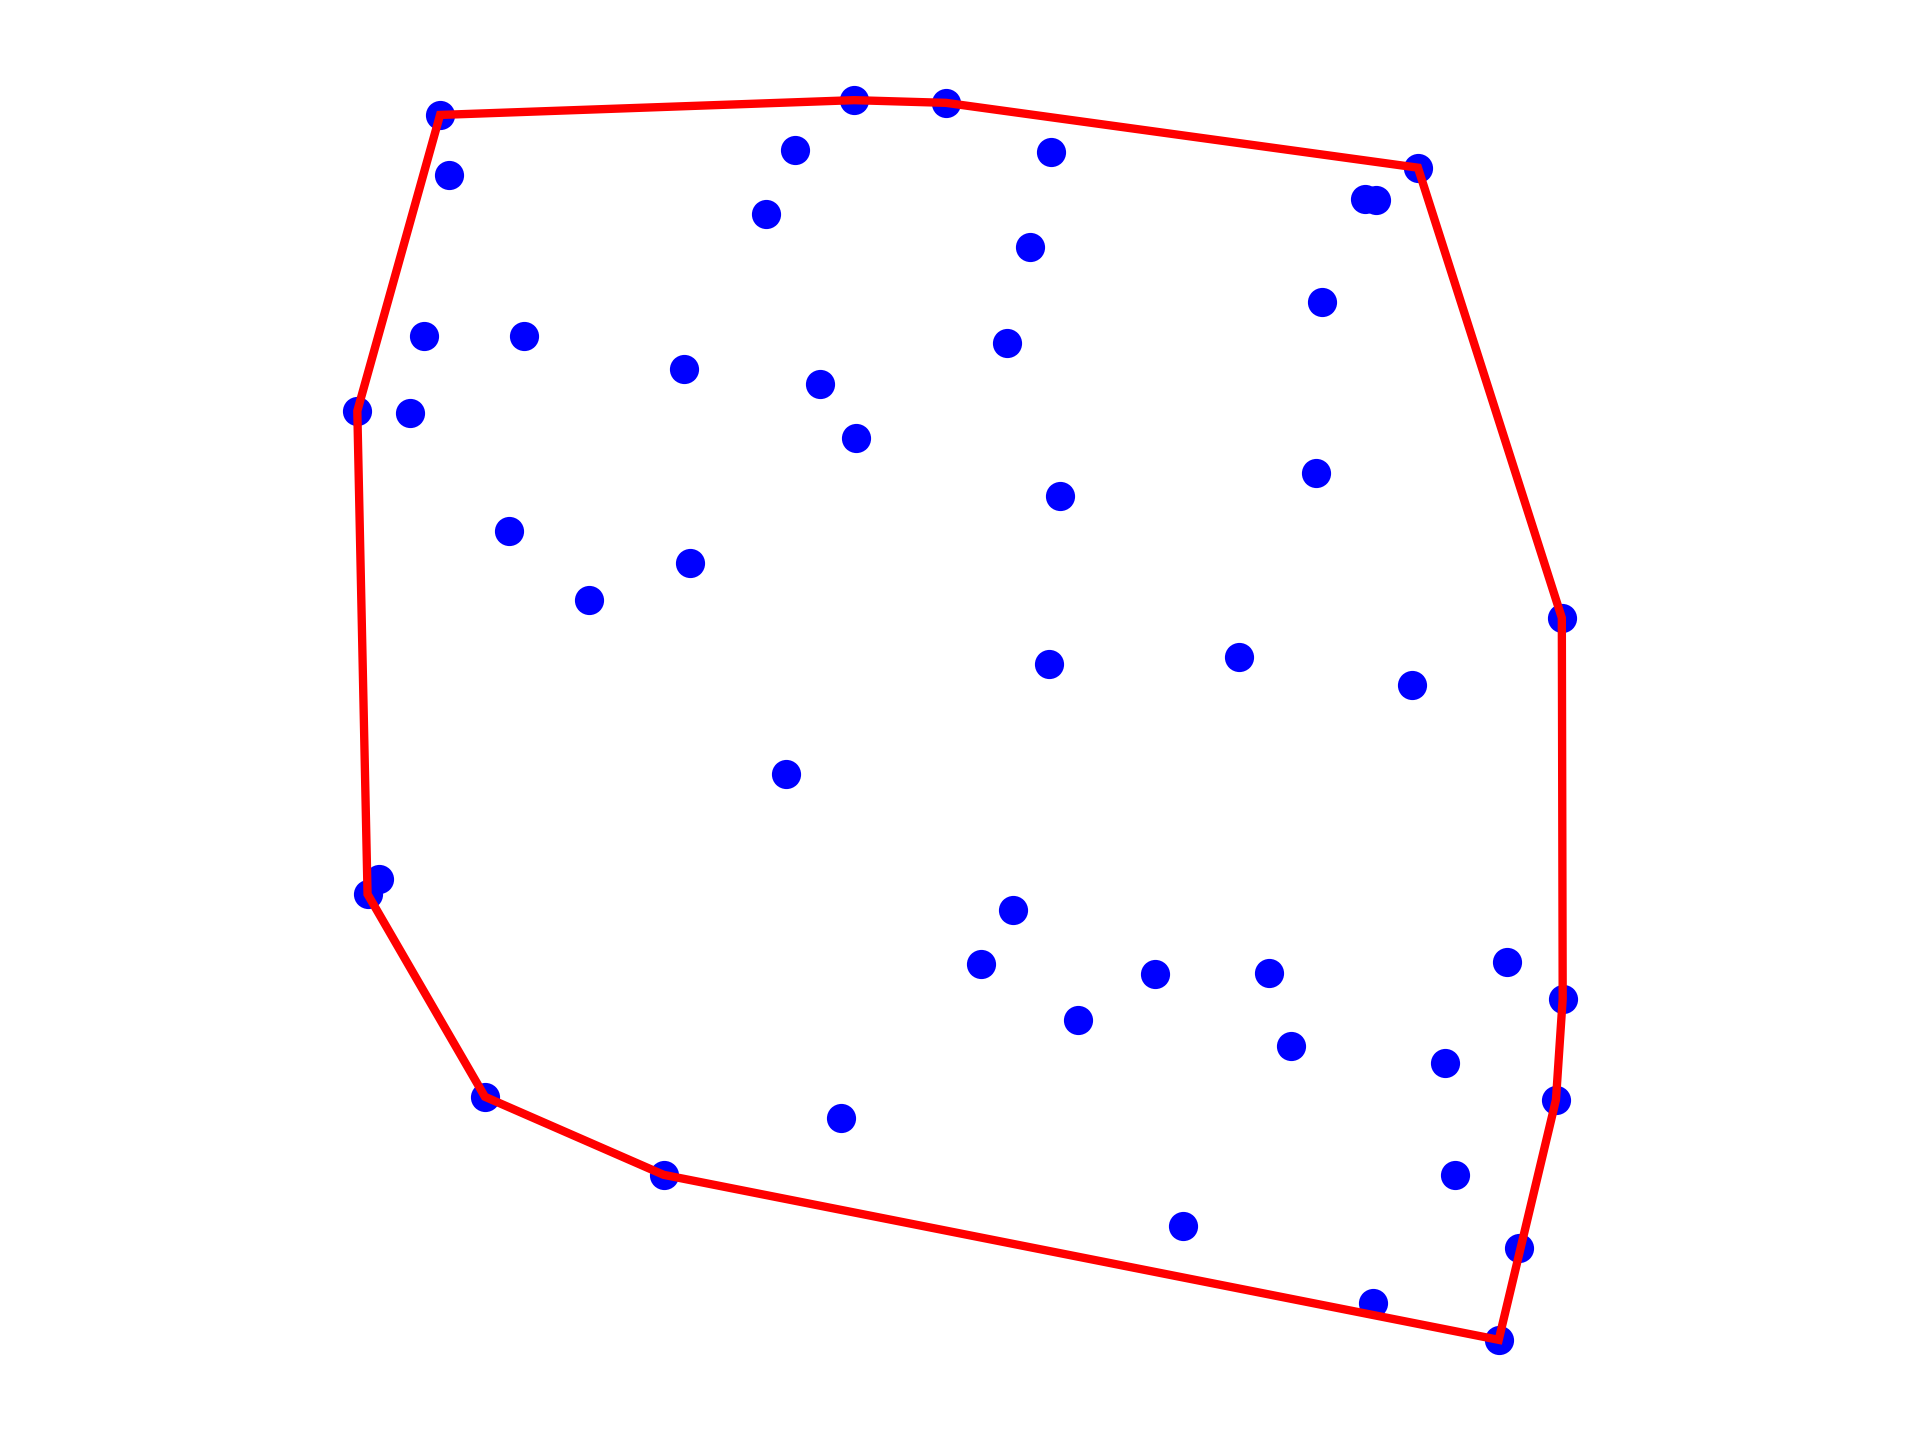
\includegraphics[scale=\myscale,scale=0.6]{figures/enveloppe}
\end{center}

\bigskip
	
Voici les étapes pour trouver le second segment de l'enveloppe convexe :
(a) on suppose que $P_1$ et $P_2$ sont déjà obtenus, on prend un point $P$ au hasard parmi les points restants ; 
(b) si un autre point $Q$ est du côté droit de la droite orientée $(\vec{P_2P})$ alors on conserve $P$ ;
(c) et (d) si par contre $Q$ est du côté gauche de $(\vec{P_2P})$ alors $Q$ devient le nouveau point $P$ ;
(e) le dernier point $P$ ainsi obtenu est le point $P_3$ qui donne le second segment de l'enveloppe convexe.

\myfigure{0.5}{
	\tikzinput{triangulation-10a}\qquad
	\tikzinput{triangulation-10b}\qquad
	\tikzinput{triangulation-10c}
	
	\medskip\medskip
	
	\tikzinput{triangulation-10d}\qquad\qquad
	\tikzinput{triangulation-10e}				
}	


Comment décider si un point $C$ est à droite ou à gauche de la droite orientée $(\vec{AB})$ ?
C'est très simple :
\begin{align*}
	 & C \text{ est à gauche de } (\vec{AB}) \\
\iff\quad & ABC \text{ est un triangle direct } \\
\iff\quad & \det( \vec{AB}, \vec{AC} ) > 0 \\
\iff\quad & \begin{vmatrix} x_B -x_A & x_C-x_A \\ y_B -y_A & y_C-y_A \\	\end{vmatrix} > 0 \\
\iff\quad & (x_B -x_A)(y_C-y_A) - (x_C-x_A)(y_B -y_A) > 0
\end{align*}

\myfigure{0.9}{
	\tikzinput{triangulation-11}
}

\bigskip

\textbf{Complexité.}
Discutons un peu de la vitesse de notre algorithme.
Bien sûr dans la pratique ce qui intéresse le programmeur et le joueur c'est de pouvoir afficher les images de sorte que l'animation soit fluide (par exemple 30 images par seconde).
Pour faire abstraction du matériel, l'efficacité d'un algorithme se mesure via sa \emph{complexité}, elle mesure le nombre d'opérations (ou la place en mémoire) nécessaire à l'algorithme en fonction de la taille $n$ des données de départ. On donne généralement la complexité sous la forme $O(n)$ ou $O(n^2)$\ldots où $O(n^k)$ signifie que le nombre d'opérations à effectuer est plus petit que $C n^k$ pour une certaine constante $C$ (que l'on ne cherche pas à connaître en général). On peut aussi distinguer la complexité dans le pire des cas ou la complexité en moyenne.

Notre algorithme a une complexité de $O(n^2)$ : il faut de l'ordre de $n^2$ opérations (ici des calculs de déterminants $2\times 2$).
En effet il faut comparer chaque point $P_i$ (au plus $n$ choix) avec tous les autres points (encore $n$ choix).
Si $n$ est petit (par exemple $n=100$) alors trouver un meilleur algorithme n'est pas important, mais si $n$ est beaucoup plus grand, ou si les calculs doivent se répéter 30 fois par seconde, alors trouver des algorithmes optimaux est important.
Par exemple pour ce problème d'enveloppe convexe, les meilleurs algorithmes sont de complexité $O(n\log n)$ ce qui est une nette amélioration lorsque $n$ est grand.


%--------------------------------------------------------------------
\subsection{Triangulation d'un ensemble de points}

Considérons maintenant le problème de la triangulation d'un ensemble $\mathcal{E}$ de points.
Il s'agit de trouver une triangulation telle que les points de $\mathcal{E}$ soient exactement l'ensemble des sommets des triangles. On exige aussi que le bord de cette triangulation soit un polygone convexe.


\myfigure{0.8}{
	\tikzinput{triangulation-12}
}


Nous faisons de nouveau une hypothèse que les points sont en position générale : c'est-à-dire que trois points ne sont jamais alignés.
On peut aussi supposer qu'il existe des points à l'intérieur de l'enveloppe convexe (sinon on renvoie à la triangulation d'un polygone convexe).

\index{algorithme!de triangulation}

\begin{algorithme}	
\textbf{Algorithme de triangulation élémentaire.}

\textbf{Entrée :} un ensemble de points $\mathcal{E}$.

\textbf{Sortie :} une liste de triplets formant une triangulation.

\begin{itemize}
	\item On calcule l'enveloppe convexe de $\mathcal{E}$.
	\item On choisit au hasard un point intérieur $P \in \mathcal{E}$. On trace les segments reliant $P$ aux sommets de l'enveloppe convexe.
	\item Pour les autres points intérieurs $Q \in \mathcal{E}$:
	\begin{itemize}
		\item on relie $Q$ aux sommets du triangle qui le contient.
	\end{itemize}	
\end{itemize}
\end{algorithme}
	
Ci-dessous à gauche une triangulation de $10$ points et à droite de $30$ points.
On voit que via notre algorithme certains triangles sont très pointus et que beaucoup sont issus d'un même sommet (le point $P$ de l'algorithme).
\begin{center}
	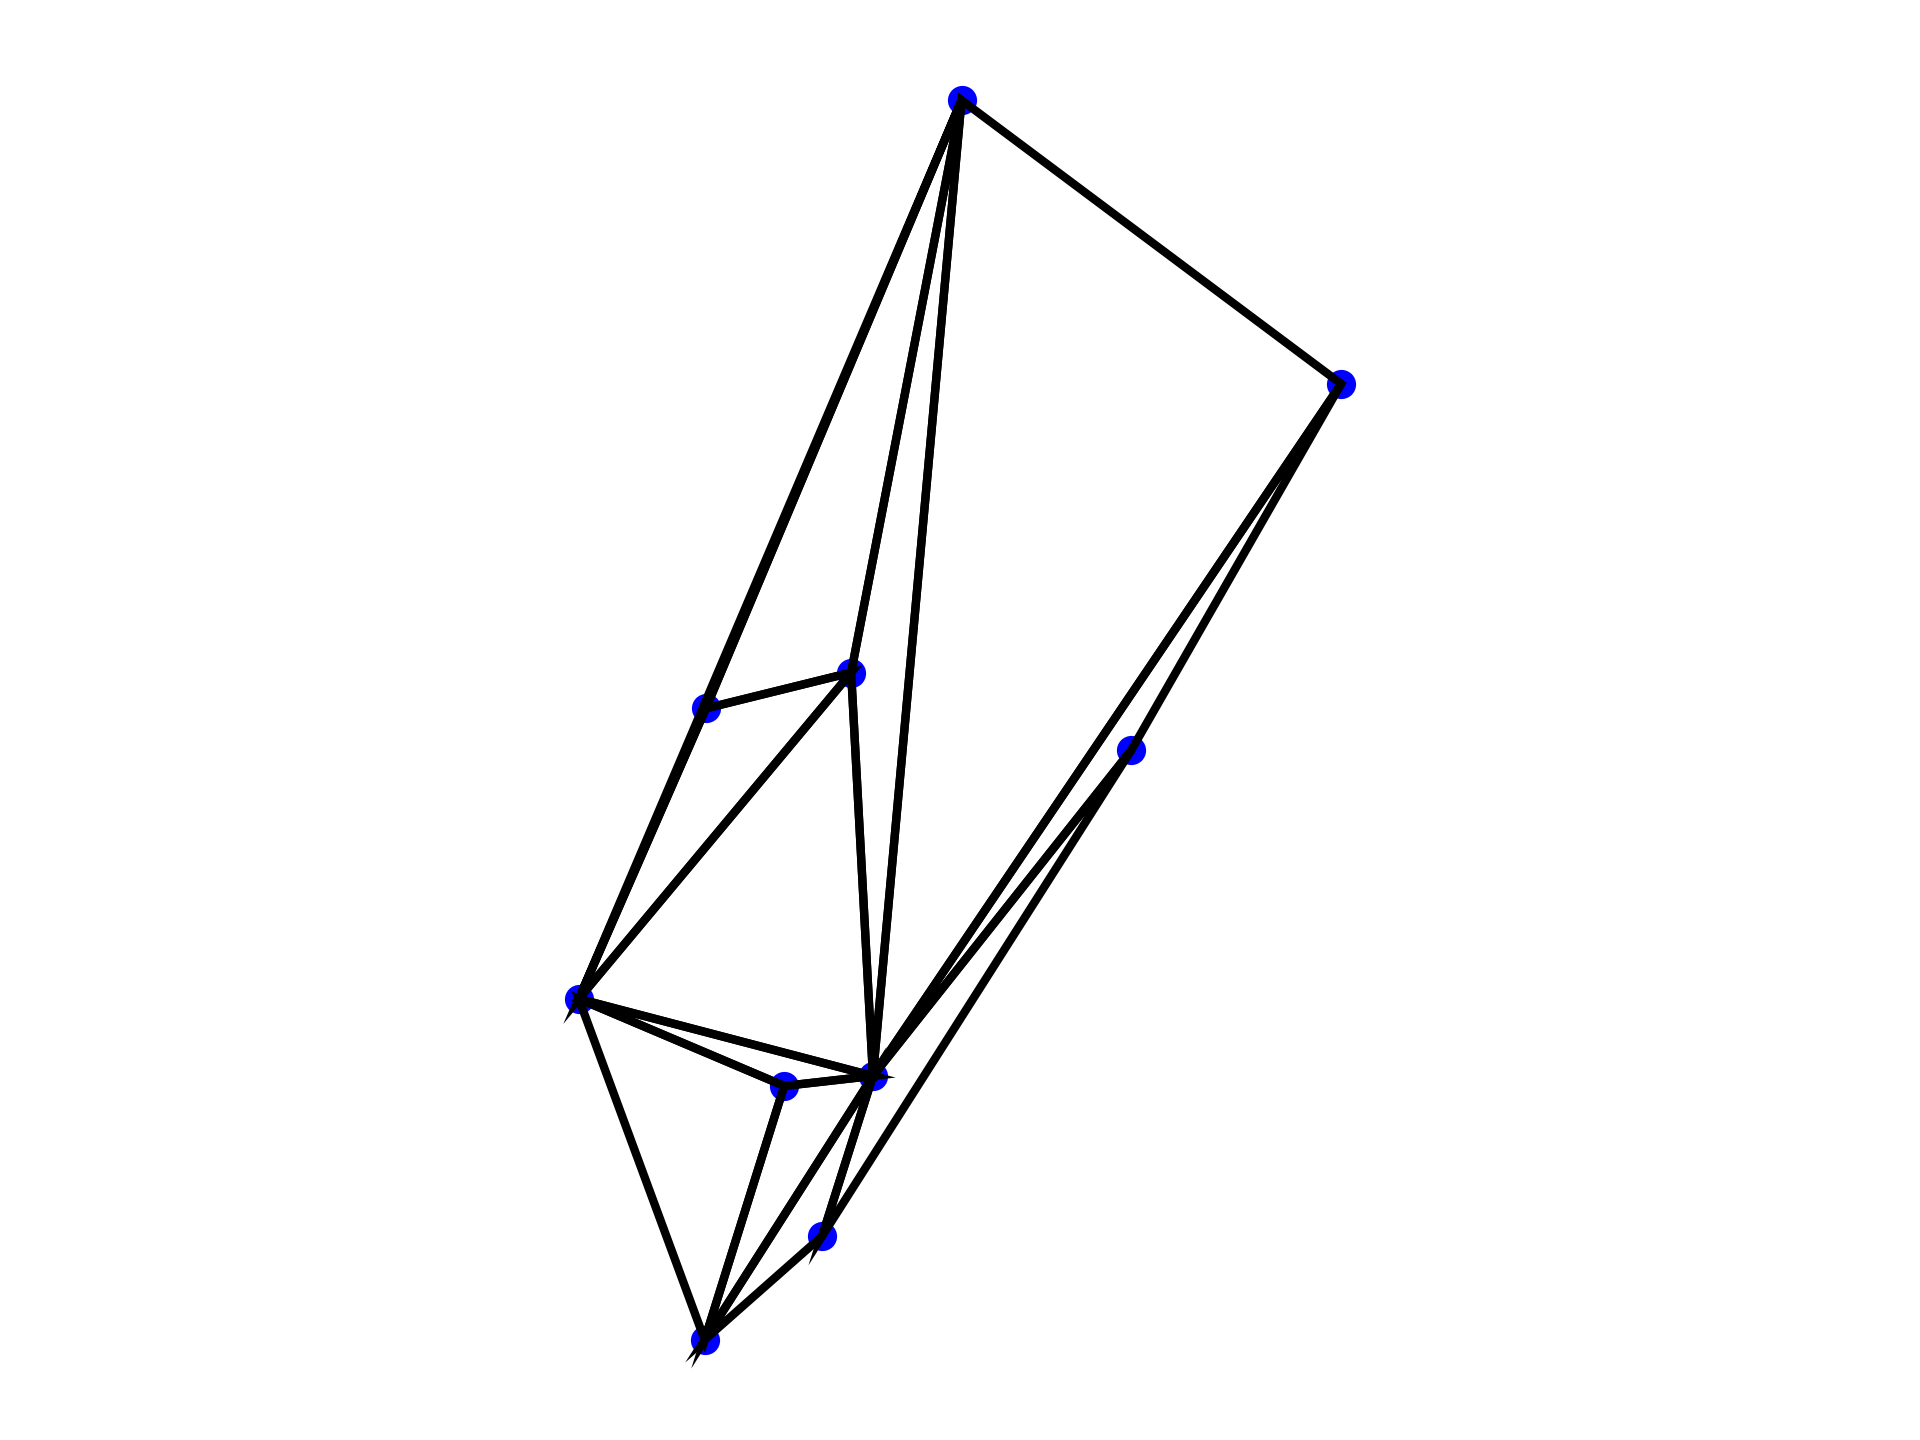
\includegraphics[scale=\myscale,scale=0.4]{figures/triangulation01}
	\qquad
	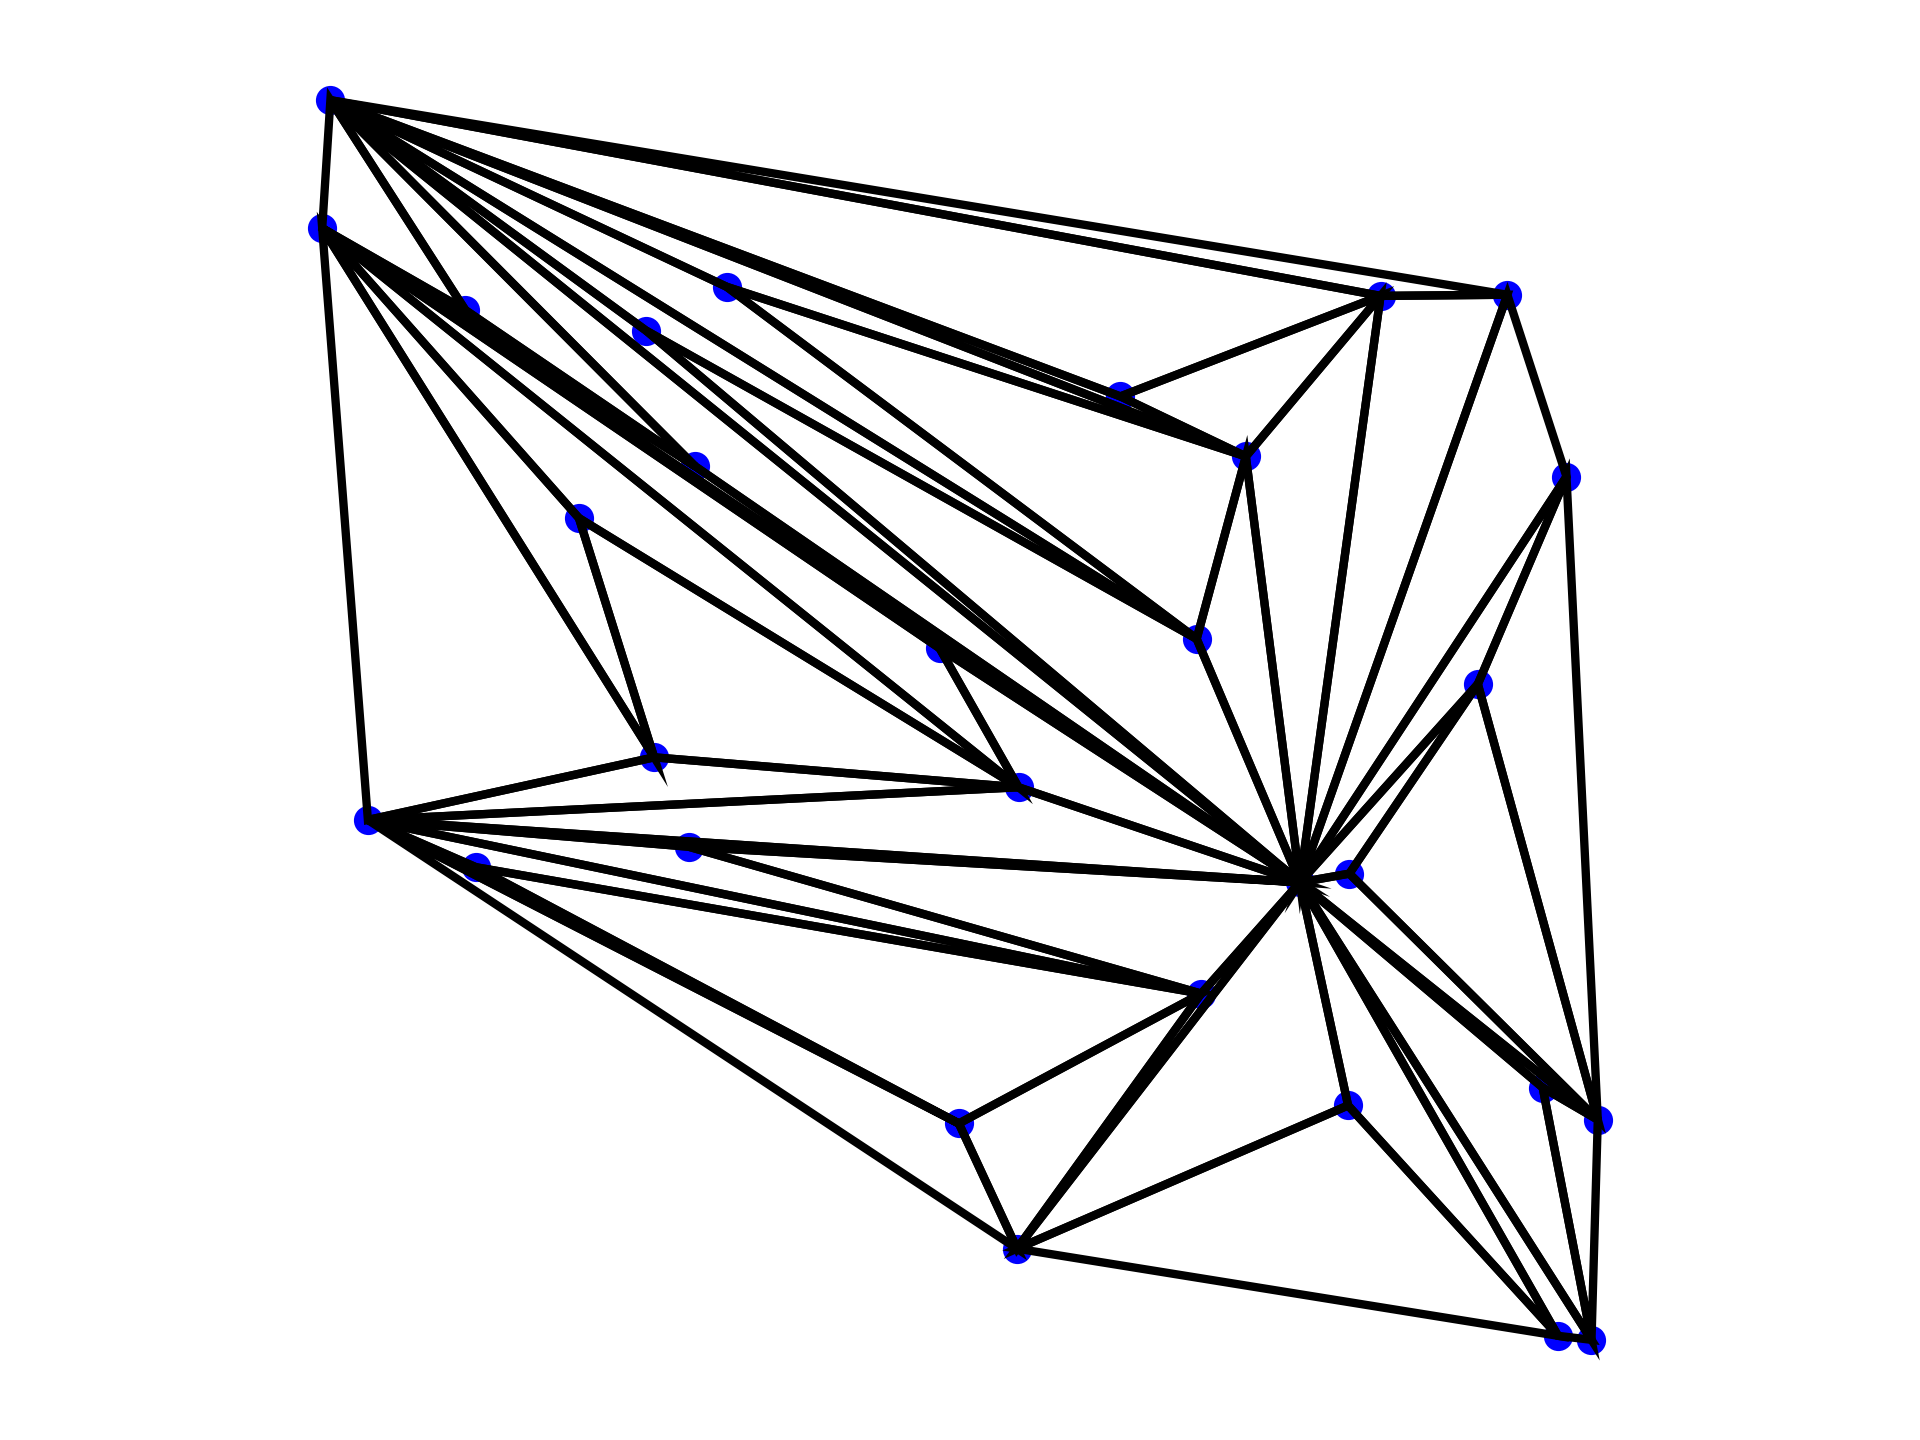
\includegraphics[scale=\myscale,scale=0.4]{figures/triangulation02}	
\end{center}


Voici les étapes de l'algorithme.

\myfigure{0.8}{
	\tikzinput{triangulation-13a}\qquad\qquad
	\tikzinput{triangulation-13b}
	
	\bigskip
	
	\tikzinput{triangulation-13c}\qquad\qquad
	\tikzinput{triangulation-13d}				
}





Il y a plusieurs précisions à apporter.

\emph{Comment encoder une triangulation ?}
On encode les points de $\mathcal{E}$ par une liste $(P_1,P_2,\ldots,P_n)$ où chaque $P_i = (x_i,y_i)$ est un couple de coordonnées.
On encode un triangle comme un triplet $(i,j,k)$ correspondant au triangle $P_iP_jP_k$, on note $\mathcal{T}$ l'ensemble de ces triplets.
La triangulation est donc $(\mathcal{E},\mathcal{T})$.

\myfigure{0.8}{
	\tikzinput{triangulation-14}
}


\bigskip

\emph{Comment déterminer si un point est à l'intérieur d'un triangle ?}
Considérons un triangle $ABC$. Pour savoir si un point $P$ est à l'intérieur du triangle on calcule ses coordonnées barycentriques
$P(\alpha:\beta:\gamma)$ (avec $\alpha+\beta+\gamma=1$).
$P$ est à l'intérieur du triangle si et seulement si $\alpha\ge0$, $\beta\ge0$ et $\gamma\ge0$.
On peut même préciser qu'il est sur un des côtés du triangle si $\alpha=0$ ou $\beta=0$ ou $\gamma=0$.
\myfigure{0.7}{
	\tikzinput{triangulation-15}\qquad\qquad\qquad
	\tikzinput{triangulation-16}	
}

On renvoie au chapitre \og{}Texture\fg{} pour les détails:
$$\alpha = \frac{\mathcal{A}_{\triangle}(PBC)}{\mathcal{A}_{\triangle}(ABC)}
\qquad
\beta = \frac{\mathcal{A}_{\triangle}(PCA)}{\mathcal{A}_{\triangle}(ABC)}
\qquad
\gamma = \frac{\mathcal{A}_{\triangle}(PAB)}{\mathcal{A}_{\triangle}(ABC)}$$
Et l'aire d'un triangle se calcule par la formule:
$$\mathcal{A}_{\triangle} (ABC) = \frac12 \left| \det(\vec{AB}, \vec{AC}) \right|$$

\myfigure{0.7}{
	\tikzinput{triangulation-17}\qquad\qquad\qquad
	\tikzinput{triangulation-18}		
}

\bigskip

\emph{Que faire dans le cas où certains points sont alignés ?}
Dans la situation précédente on part d'un point $P$ à l'intérieur d'un triangle, et on remplace ce triangle par trois nouveaux triangles.Si par contre $P$ est sur un côté bordant deux triangles, alors on remplace ces triangles par quatre nouveaux triangles.


\myfigure{0.5}{
	\tikzinput{triangulation-19}
}

\myfigure{0.5}{	
	\tikzinput{triangulation-20}		
}


\bigskip

\emph{Une triangulation est-elle unique ?} Non, il y a énormément de triangulations possibles.
Par contre, quelle que soit la triangulation, le nombre de triangles reste le même.

\begin{proposition}
	Soit $\mathcal{E}$ un ensemble de $n$ points, dont l'enveloppe convexe contient $b$ points.
	Le nombre de triangles d'une triangulation de $\mathcal{E}$ est $2n-b-2$.
	Le nombre d'arêtes est $3n-b-3$.
\end{proposition}	

\begin{proof}
Le nombre de sommets est $S = n$.
Le nombre de faces est $F = t+1$ où $t$ est le nombre de triangles et où on n'oublie pas la face non bornée.
Notons $A$ le nombre d'arêtes.
Si on considère une arête interne alors elle est le bord de deux triangles.
Réciproquement un triangle est bordé par trois arêtes. Donc si on compte grossièrement on a deux arêtes pour trois triangles. Notre compte n'est pas tout fait juste car les arêtes du bord ne bordent qu'un seul triangle. La relation exacte est :
$$2A -b = 3t.$$


Appliquons maintenant la formule d'Euler $S-A+F=2$.
Dans cette formule on va substituer $S=n$,
et de la relation $2A-b=3t$ on tire $A=\frac{3t+b}{2}$, et enfin $F=t+1$.
Ainsi la formule d'Euler devient
$n-\frac{3t+b}{2} + t+1 = 2$. Ce qui donne la relation voulue : $t = 2n-b-2$.
Ce qui permet de calculer le nombre d'arêtes $A = 3n-b-3$.
\end{proof}


%%%%%%%%%%%%%%%%%%%%%%%%%%%%%%%%%%%%%%%%%%%%%%%%%%%%%%%%%%%%%%%%%%%%%
\section{Triangulation de Delaunay}

\index{triangulation!de Delaunay}

%--------------------------------------------------------------------
\subsection{Cercle circonscrit}

\begin{proposition}

Le cercle circonscrit $\mathcal{C}$ d'un triangle $ABC$ a pour centre
$O$ de coordonnées $(x_O,y_O)$ où :
$$x_O = \frac{1}{2\Delta}\begin{vmatrix}x_A^2+y_A^2 & y_A & 1 \\ x_B^2+y_B^2 & y_B & 1 \\ x_C^2+y_C^2 & y_C & 1 \end{vmatrix}
\qquad \text{ et } \qquad 
y_O = -\frac{1}{2\Delta}\begin{vmatrix}x_A^2+y_A^2 & x_A & 1 \\ x_B^2+y_B^2 & x_B & 1 \\ x_C^2+y_C^2 & x_C & 1 \end{vmatrix}
\qquad \text{ avec } \qquad
\Delta= \begin{vmatrix}x_A & y_A & 1 \\ x_B & y_B & 1 \\ x_C & y_C & 1 \end{vmatrix}
$$
et a pour rayon 
$r = OA = \sqrt{ (x_A-x_O)^2 + (y_A-y_O)^2 }$.
\end{proposition}	

\myfigure{0.6}{	
	\tikzinput{delaunay-01}		
}



\begin{proposition}
Soit $ABC$ un triangle \emph{direct}.
Un point $P(x,y)$ est sur le bord ou à l'intérieur du cercle $\mathcal{C}$ si et seulement si :
$$\begin{vmatrix}
	x^2+y^2     & x   & y   & 1 \\
	x_A^2+y_A^2 & x_A & y_A & 1 \\ 
	x_B^2+y_B^2 & x_B & y_B & 1 \\ 
	x_C^2+y_C^2 & x_C & y_C & 1 
\end{vmatrix} \le 0$$
\end{proposition}
Dans le cas d'un triangle indirect, le point $P$ est à l'intérieur de $\mathcal{C}$ si le déterminant est positif.

\myfigure{0.5}{	
	\tikzinput{delaunay-02}		
}


Considérons un quadrilatère convexe de sommets $A$, $B$, $C$, $D$ comme sur la figure ci-dessous.

\begin{itemize}
	\item On dit que la diagonale $[BC]$ est \defi{bonne} si le cercle $\mathcal{C}_1$ circonscrit à $ABC$ ne contient pas le point $D$ dans son intérieur
et si le cercle $\mathcal{C}_2$ circonscrit à $BCD$ ne contient pas le point $A$ dans son intérieur.

\myfigure{0.6}{	
	\tikzinput{delaunay-03}		
}

    \item Dans le cas contraire on dit que la diagonale $[BC]$ est \defi{mauvaise} : soit le cercle $\mathcal{C}_1$ circonscrit à $ABC$ contient le point $D$ dans son intérieur
    ou bien le cercle $\mathcal{C}_2$ circonscrit à $BCD$ contient le point $A$ dans son intérieur.
    
\myfigure{0.5}{	
	\tikzinput{delaunay-04}		
}


\end{itemize}




\begin{proposition}[Mauvaise arête et basculement]
Considérons un quadrilatère convexe de sommets $A$, $B$, $C$, $D$.
Soit la diagonale $[BC]$ est bonne, soit la diagonale $[AD]$ est bonne.
\end{proposition}

\myfigure{0.5}{	
	\tikzinput{delaunay-03bis}		
}

L'une des deux diagonales est donc une bonne diagonale.
Autrement dit, les deux diagonales ne peuvent être mauvaises simultanément.
Le seul cas où les deux diagonales sont bonnes en même temps est lorsque les points $A$, $B$, $C$, $D$ sont cocycliques.

\myfigure{0.45}{	
	\tikzinput{delaunay-05}		
}


%--------------------------------------------------------------------
\subsection{Triangulation de Delaunay}

\begin{definition}
	Soit $\mathcal{E}$ un ensemble de points.
	On dit qu'une triangulation $\mathcal{T}$ est une \defi{triangulation de Delaunay} de $\mathcal{E}$
	si pour tout triangle $T$ de $\mathcal{T}$, le cercle circonscrit à $T$ ne contient aucun point de $\mathcal{E}$ dans son intérieur strict.
\end{definition}	

Le premier point fort d'une triangulation de Delaunay est qu'il n'y en a (presque) qu'une seule.
\begin{theoreme}
Pour n'importe quel ensemble fini de points, il existe une triangulation de Delaunay.
De plus cette triangulation est unique, à l'exception des sommets cocycliques où un basculement fournit deux possibilités.
\end{theoreme}

\myfigure{0.5}{	
	\tikzinput{delaunay-06}		
}


Ci-dessous une triangulation de Delaunay de $20$ points (à gauche) et de $100$ points(à droite) .
\begin{center}
	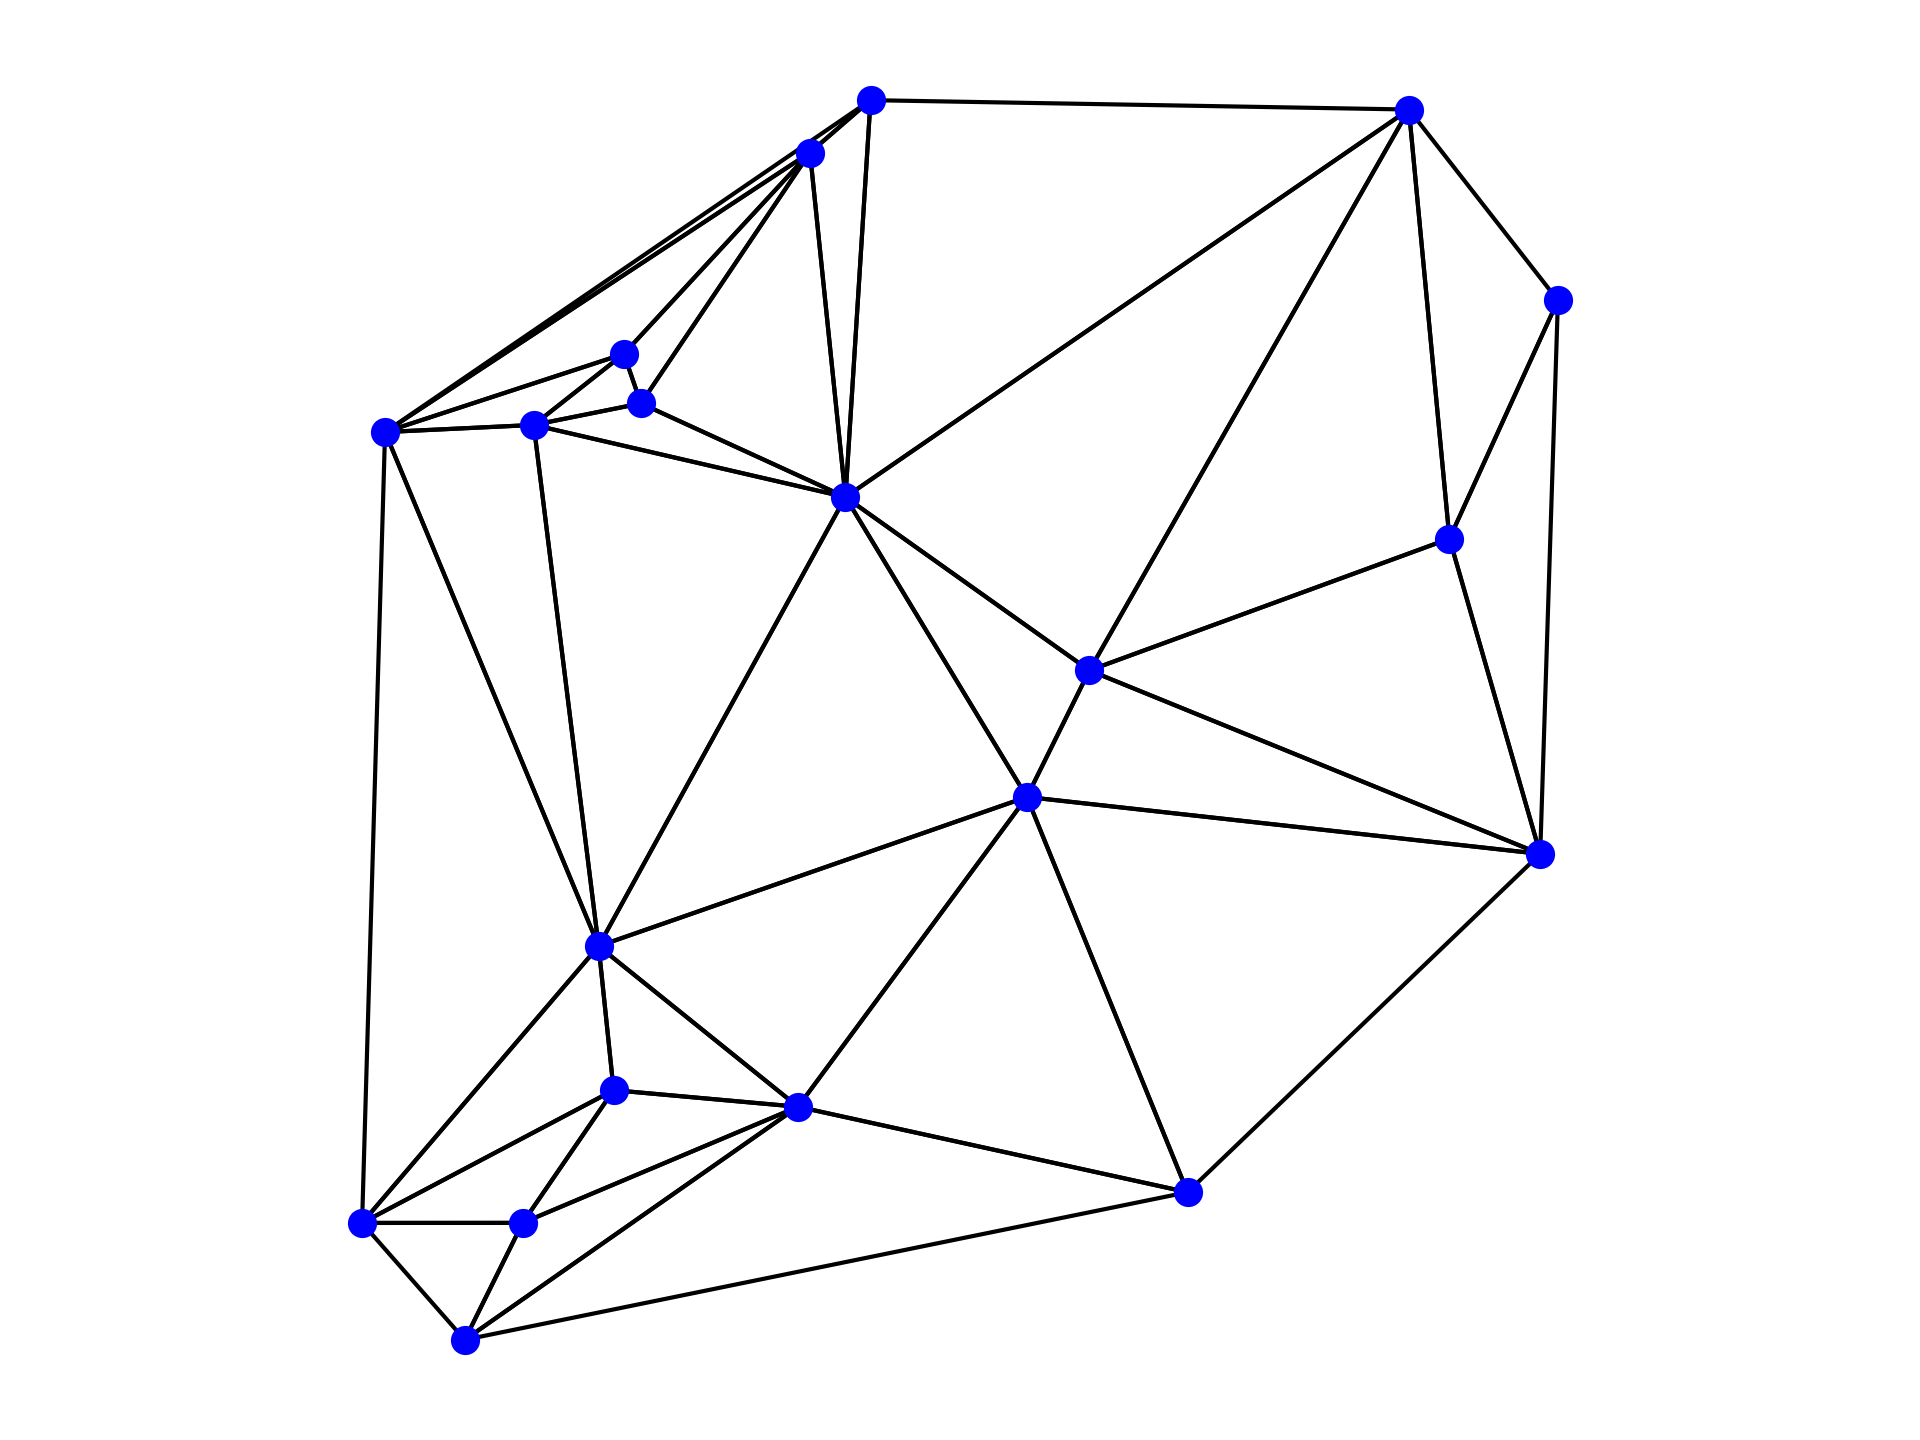
\includegraphics[scale=\myscale,scale=0.4]{figures/delaunay01}
	\qquad
	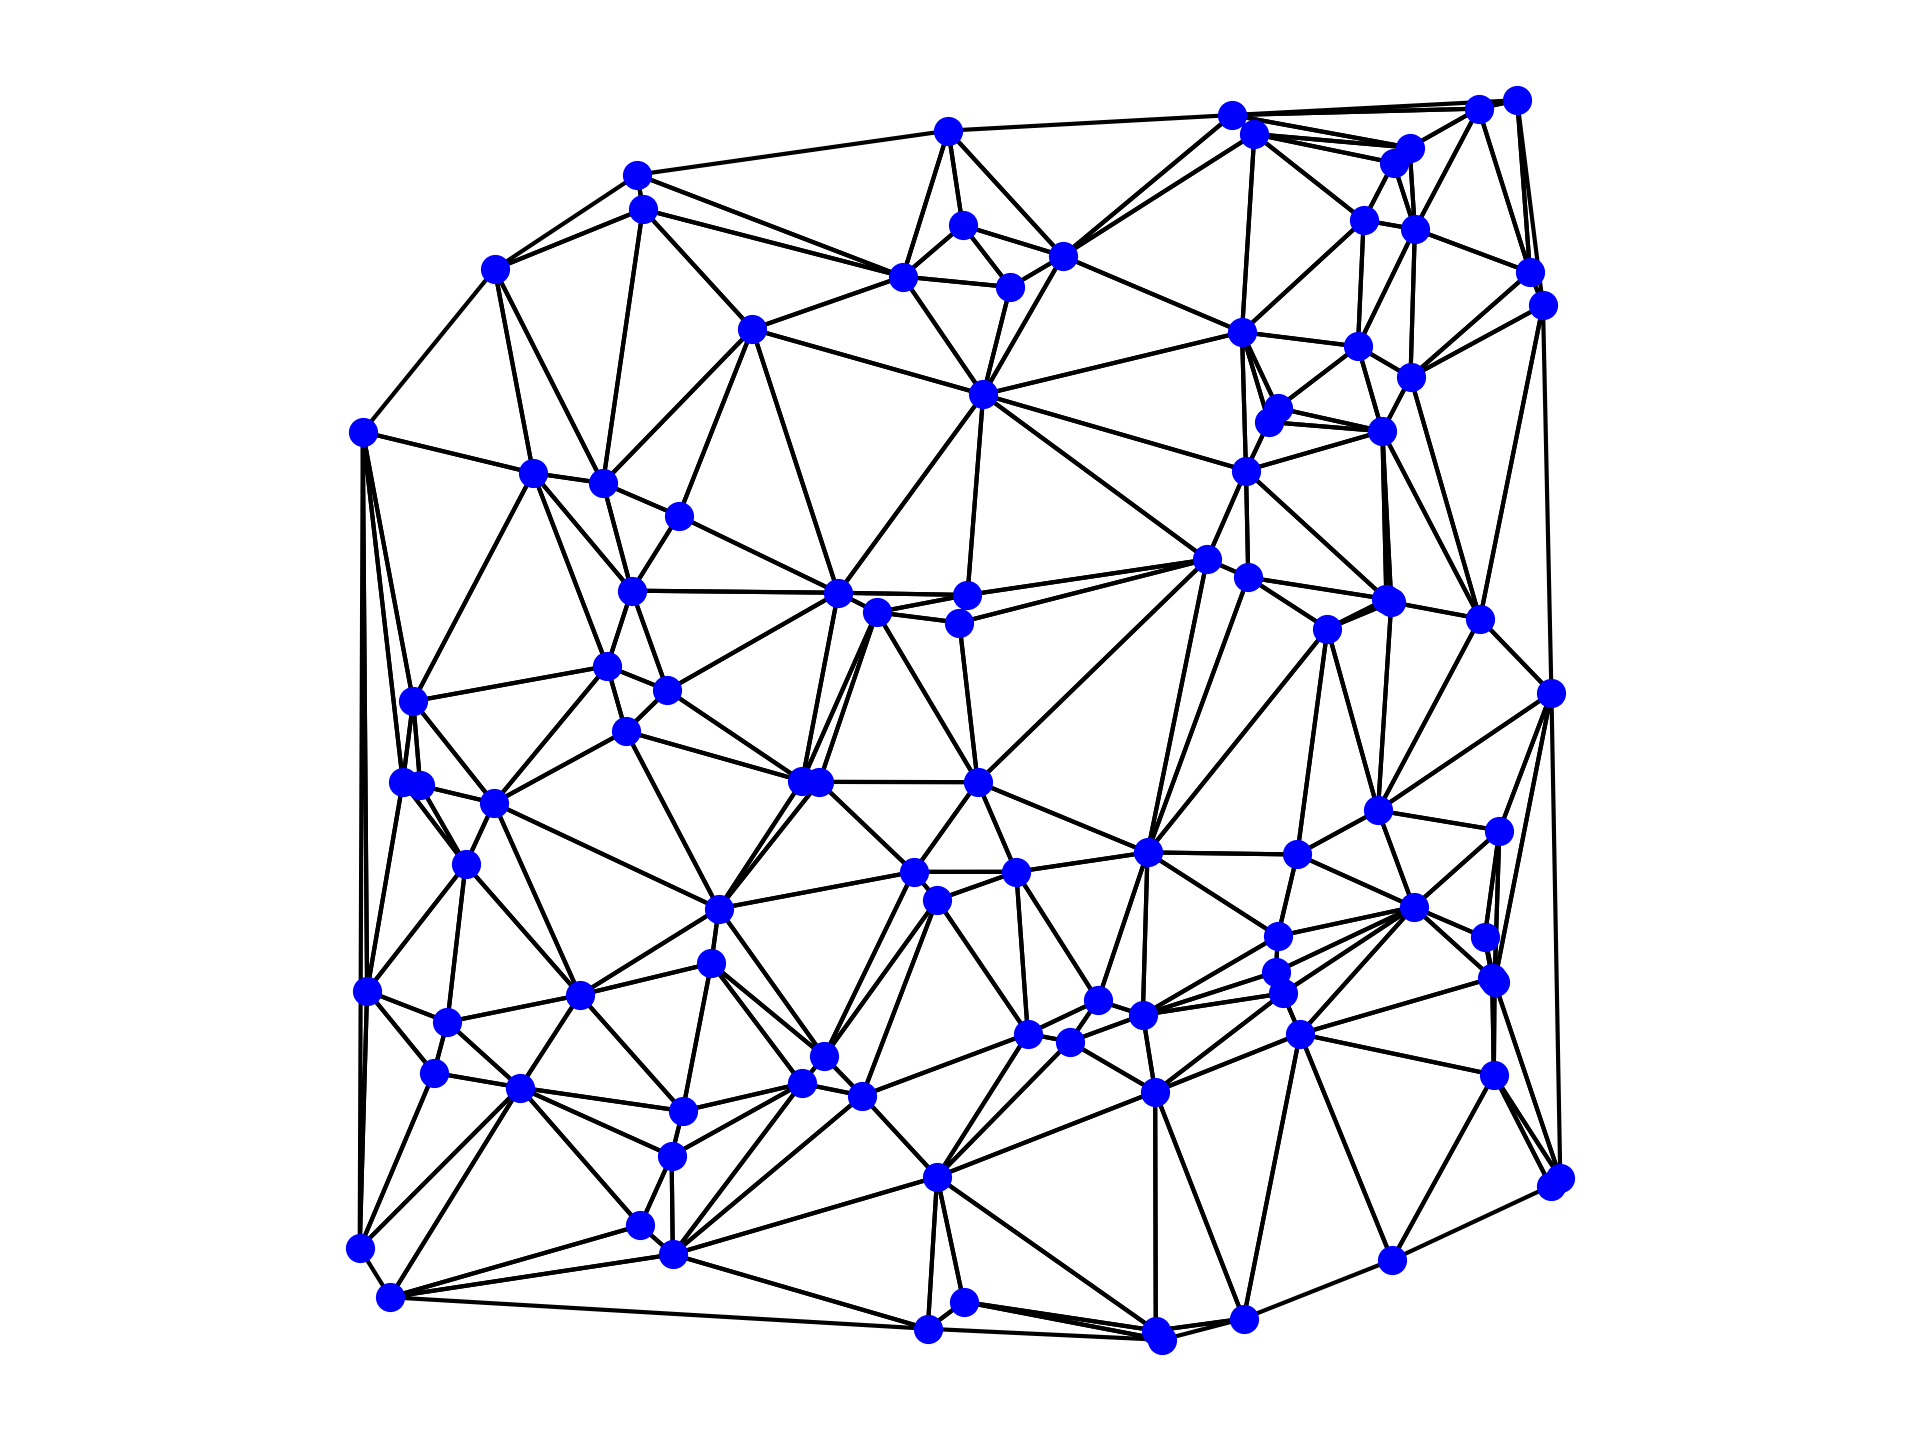
\includegraphics[scale=\myscale,scale=0.4]{figures/delaunay02}	
\end{center}

\bigskip

Pourquoi une triangulation de Delaunay serait-elle meilleure qu'une autre ?
La triangulation de Delaunay est celle qui évite le mieux les triangles ayant des angles très aigus, c'est-à-dire les petits angles où le triangle est pointu.
Bien sûr on ne peut pas toujours éviter les triangles pointus mais la triangulation de Delaunay est celle qui le fait le mieux (elle réalise un minimum global d'une certaine fonction évaluant tous les angles de tous les triangles).

Le basculement s'explique bien avec cette notion d'angle, lorsque l'on bascule une arête d'un quadrilatère, la seule chose qui change ce sont les $6$ angles.
Lorsque l'on bascule une mauvaise arête, alors l'angle le plus petit avant basculement est plus petit que l'angle le plus petit après :
$\min_{i=1,\ldots,6} \alpha_i < \min_{i=1,\ldots,6} \beta_i$.


\myfigure{0.7}{	
	\tikzinput{delaunay-07}		
}


%--------------------------------------------------------------------
\subsection{Algorithme par basculement}

Rappelons que dans un quadrilatère, si l'arête diagonale est mauvaise, on peut toujours la transformer en une bonne arête par \defi{basculement}\index{triangulation!basculement}. Cela va nous permettre de calculer une triangulation de Delaunay à partir d'une triangulation quelconque.

\myfigure{0.5}{	
	\tikzinput{delaunay-08}		
}

\index{algorithme!de triangulation}

\begin{algorithme}
\textbf{Algorithme de basculement.}

\textbf{Entrée :} un ensemble de points $\mathcal{E}$ muni d'une triangulation $\mathcal{T}$.

\textbf{Sortie :} la triangulation de Delaunay de $\mathcal{E}$.

\begin{itemize}
	\item Tant qu'il existe un quadrilatère avec une mauvaise diagonale :
	\begin{itemize}
		\item basculer cette arête en une bonne diagonale.
	\end{itemize} 
\end{itemize}	  	
\end{algorithme}
	
\bigskip



L'algorithme est donc très simple. Voici un exemple :

\myfigure{0.5}{	
	\tikzinput{delaunay-09b}\qquad\qquad\qquad		
	\tikzinput{delaunay-09c}
	
	\bigskip
	
	\tikzinput{delaunay-09d}\qquad\qquad\qquad
	\tikzinput{delaunay-09e}
	
    \bigskip	
	
	\tikzinput{delaunay-09f}\qquad\qquad\qquad
	\tikzinput{delaunay-09g}
						
}

Reprenez cet ensemble de points, dessinez une autre triangulation, appliquez l'algorithme : vous devez obtenir la même triangulation finale !



Il y a quand même des subtilités : en cours d'exécution de l'algorithme le caractère bon ou mauvais d'une diagonale peut changer, en effet les triangles (donc les quadrilatères) changent au fil de l'algorithme, il ne s'agit donc pas de calculer toutes les mauvaises diagonales au départ et de les basculer. L'algorithme cherche une mauvaise diagonale, la bascule, puis cherche une mauvaise diagonale dans la nouvelle triangulation\ldots

Vu la remarque précédente il n'est pas évident du tout que l'algorithme se termine. Une arête que l'on vient de basculer en une bonne diagonale, peut-elle se retrouver plus tard une mauvaise diagonale ? Heureusement non, ce qui fait que l'algorithme termine toujours par une triangulation sans mauvaises diagonale, c'est-à-dire une triangulation de Delaunay.
Cet algorithme élémentaire n'est pas très rapide, sa complexité est $O(n^2)$ où $n$ est le nombre de sommets. Il existe des algorithmes de triangulation de Delaunay en $O(n)$.



%%%%%%%%%%%%%%%%%%%%%%%%%%%%%%%%%%%%%%%%%%%%%%%%%%%%%%%%%%%%%%%%%%%%%
\section{Cellules de Voronoï}

\index{cellule de Voronoi@cellule de Voronoï}

%--------------------------------------------------------------------
\subsection{La guerre des princesses}

Des princesses habitent un pays, chacune dans son château. Pour se partager le territoire en évitant de se faire la guerre elles décident de la règle suivante :  \og{}Chacune est propriétaire du terrain plus proche de son château que des autres châteaux.\fg{}


S'il y a seulement deux princesses $A$ et $B$ alors chacune contrôle un demi-plan.
La séparation se fait selon la médiatrice $[AB]$ des deux châteaux.

\myfigure{0.6}{	
	\tikzinput{voronoi-01}		
}

S'il y a trois princesses $A$, $B$, $C$ c'est déjà plus intéressant. On dessine les médiatrices du triangle $ABC$ et leur point d'intersection $O$ (qui est aussi le centre du cercle circonscrit). Les zones sont délimitées par les \og{}demi-médiatrices\fg{} issues de $O$.

\myfigure{0.7}{	
	\tikzinput{voronoi-02}		
}

La zone contrôlée par une princesse s'appelle une \defi{cellule de Voronoï}.
S'il y a $4$ princesses ou plus alors plusieurs types de configurations sont possibles. Certaines cellules de Voronoï peuvent être bornées, d'autres non.

\myfigure{0.5}{	
	\tikzinput{voronoi-03a}\qquad\qquad\qquad
	\tikzinput{voronoi-03b}		
}


\myfigure{0.7}{	
	\tikzinput{voronoi-04}		
}

Les applications sont nombreuses, par exemple les cellules vivantes se développent jusqu'à rencontrer les cellules voisines, de même un sol asséché se craquelle en cellules de Voronoï,
enfin votre téléphone se connecte à l'antenne relais la plus proche c'est-à-dire lorsque vous êtes dans sa cellule de Voronoï.


%--------------------------------------------------------------------
\subsection{Dual de Delaunay}

Tracer les cellules de Voronoï d'un ensemble de points c'est très simple à partir de la triangulation de Delaunay. Les sommets des cellules sont les centres des cercles circonscrits à chaque triangle de la triangulation. Les bords des cellules sont les portions des médiatrices de ces triangles reliant deux sommets voisins.
Les cellules de Voronoï correspondent au \emph{graphe dual} de la triangulation de Delaunay.

\begin{algorithme}
\textbf{Algorithme des cellules de Voronoï.}

\textbf{Entrée :} un ensemble de points $\mathcal{E}$.
% muni d'une triangulation $\mathcal{T}$.

\textbf{Sortie :} le graphe $\mathcal{V}$ de Voronoï de $\mathcal{E}$.

\begin{itemize}
	\item Calculer la triangulation $\mathcal{T}$ de Delaunay de $\mathcal{E}$.
	\item Les sommets de $\mathcal{V}$ sont les centres des cercles circonscrits des triangles de $\mathcal{T}$.
	\item Les arêtes de $\mathcal{V}$ sont les portions de médiatrices des côtés des triangles de $\mathcal{T}$ joignant deux sommets voisins (ou infinies s'il n'y a pas de voisin).
\end{itemize}	
\end{algorithme}
	
Voici les étapes de l'algorithme.


\myfigure{0.6}{	
	\tikzinput{voronoi-05a}\qquad\qquad
	\tikzinput{voronoi-05b}	
	
	\bigskip
	
	\tikzinput{voronoi-05c}\qquad\qquad
	\tikzinput{voronoi-05d}	
	
	\bigskip
	
	\tikzinput{voronoi-05e}			
}

\bigskip

Voici un exemple avec $10$ points. Sur la figure de gauche on a dessiné la triangulation de Delaunay \couleurnb{(en noir) }{}et sa triangulation duale \couleurnb{(en vert) }{}qui délimite les cellules de Voronoï (les demi-médiatrices infinies ne sont pas tracées). Sur la figure de droite les cellules de Voronoï de ces mêmes points. 
\begin{center}
	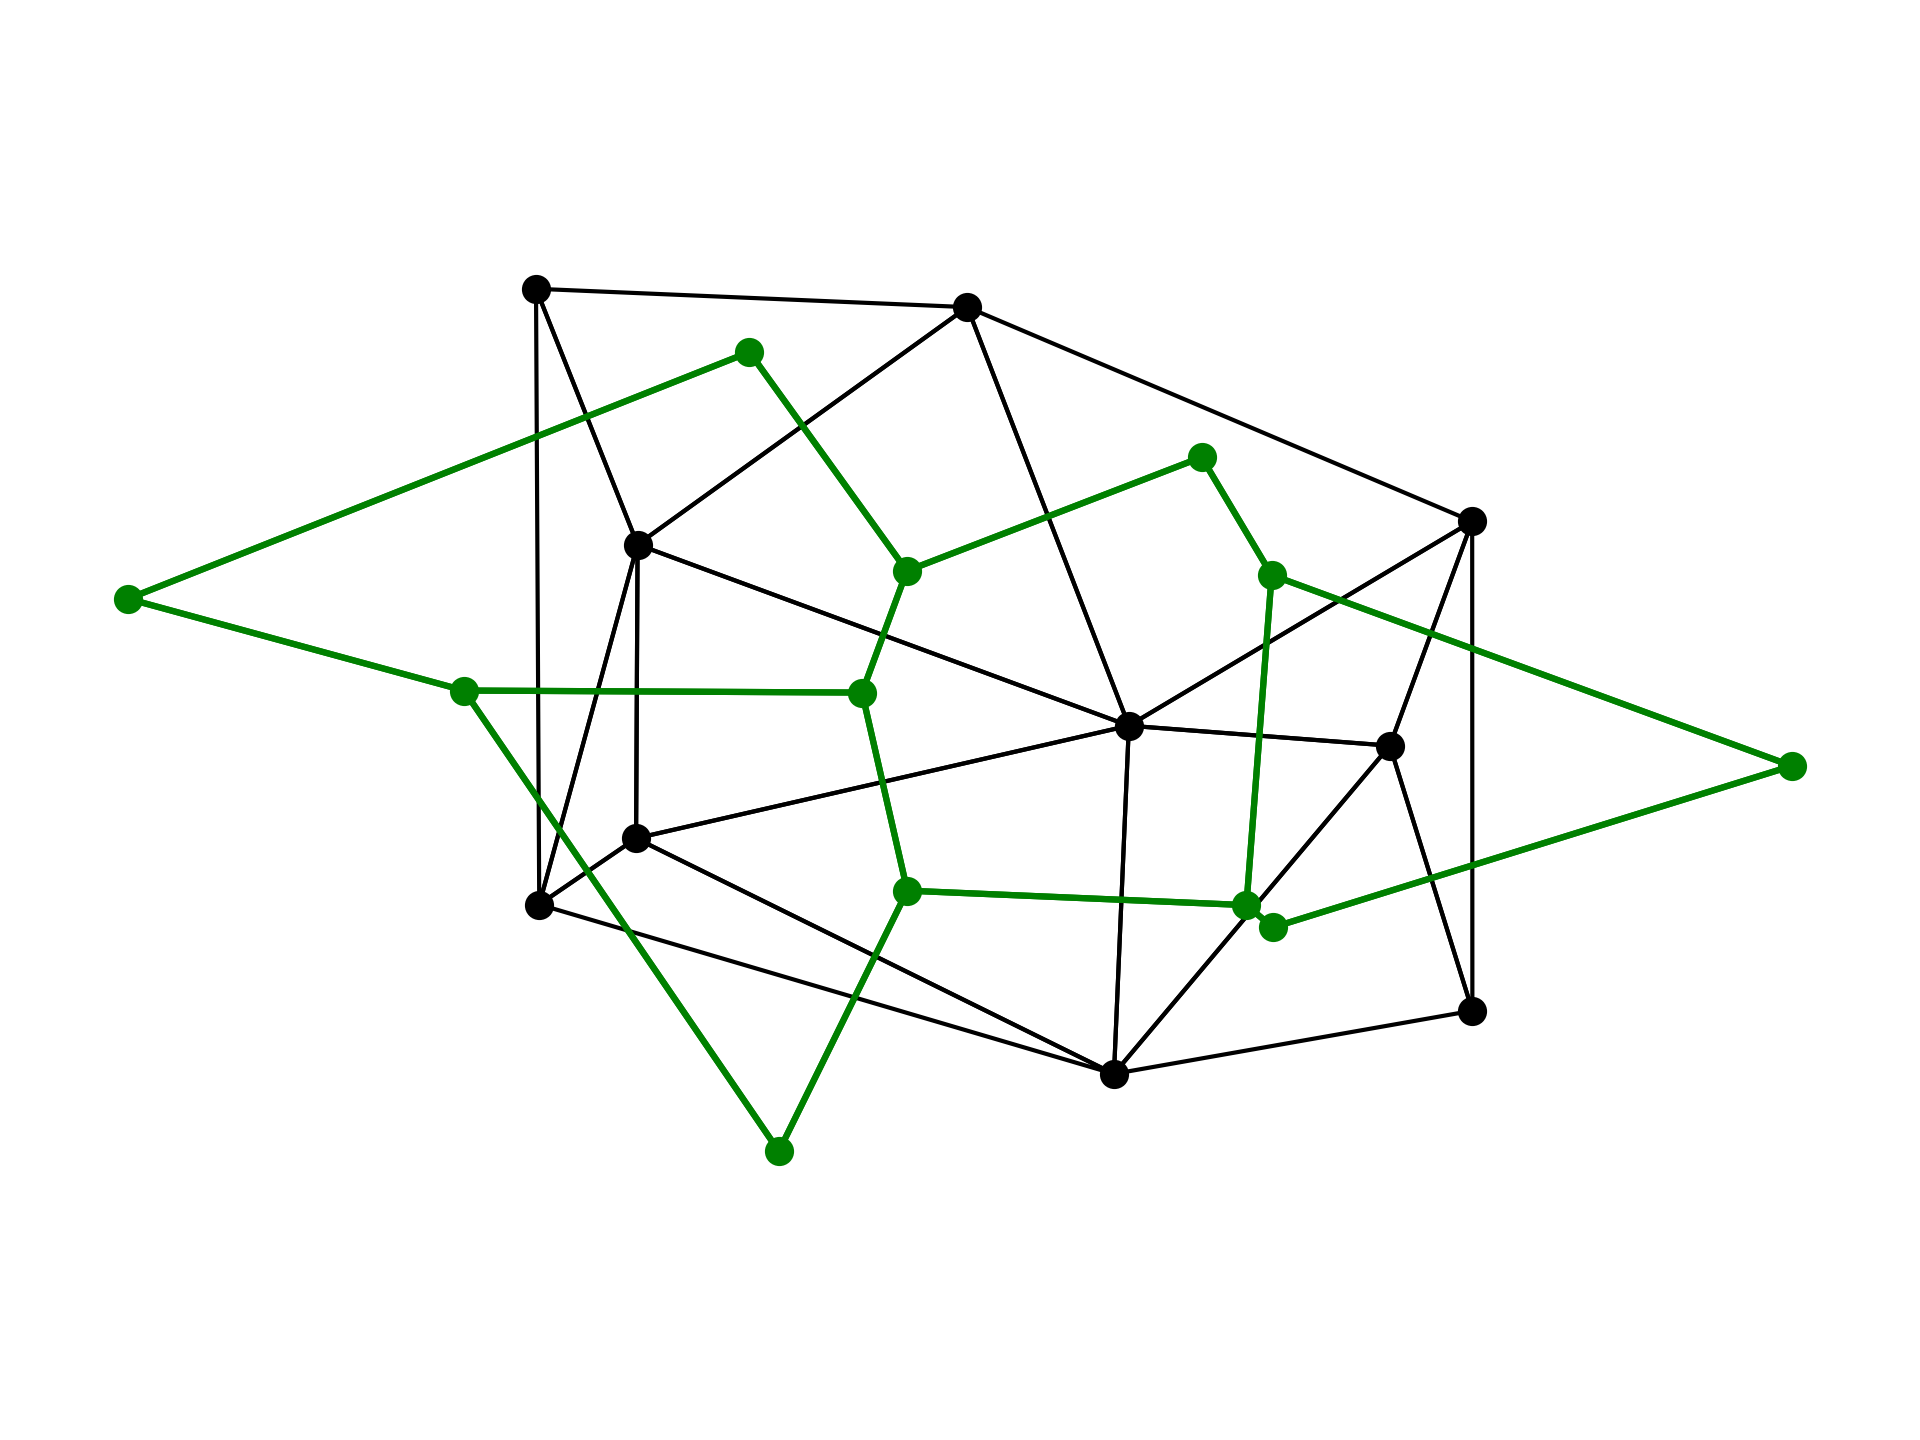
\includegraphics[scale=\myscale,scale=0.45]{figures/voronoi01a}
	\qquad
	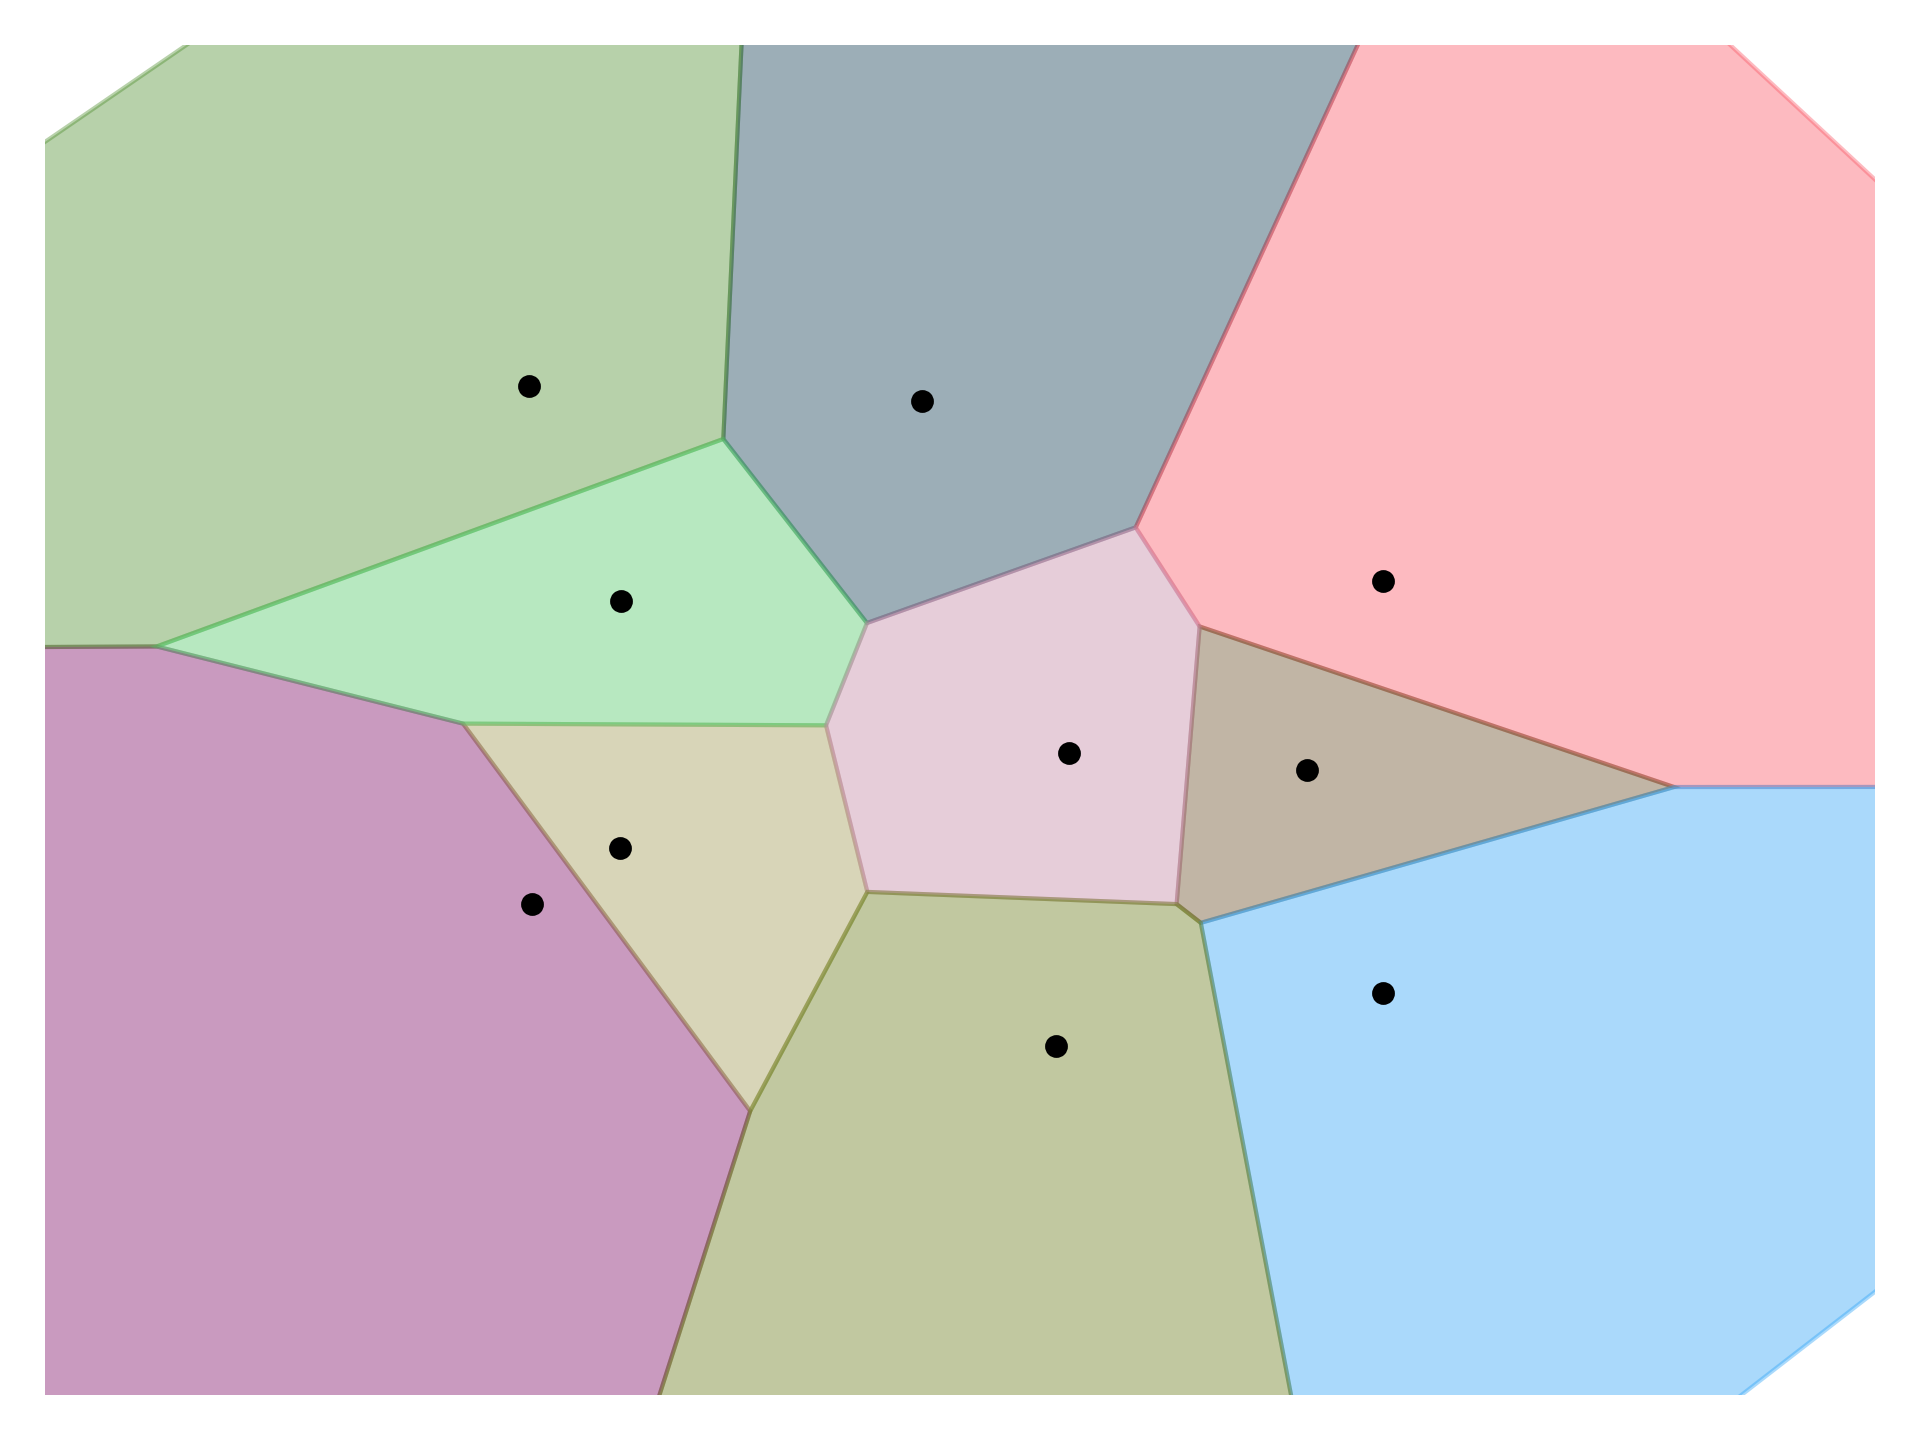
\includegraphics[scale=\myscale,scale=0.45]{figures/voronoi01b}	
\end{center}

Voici un exemple avec $100$ points.
\begin{center}
	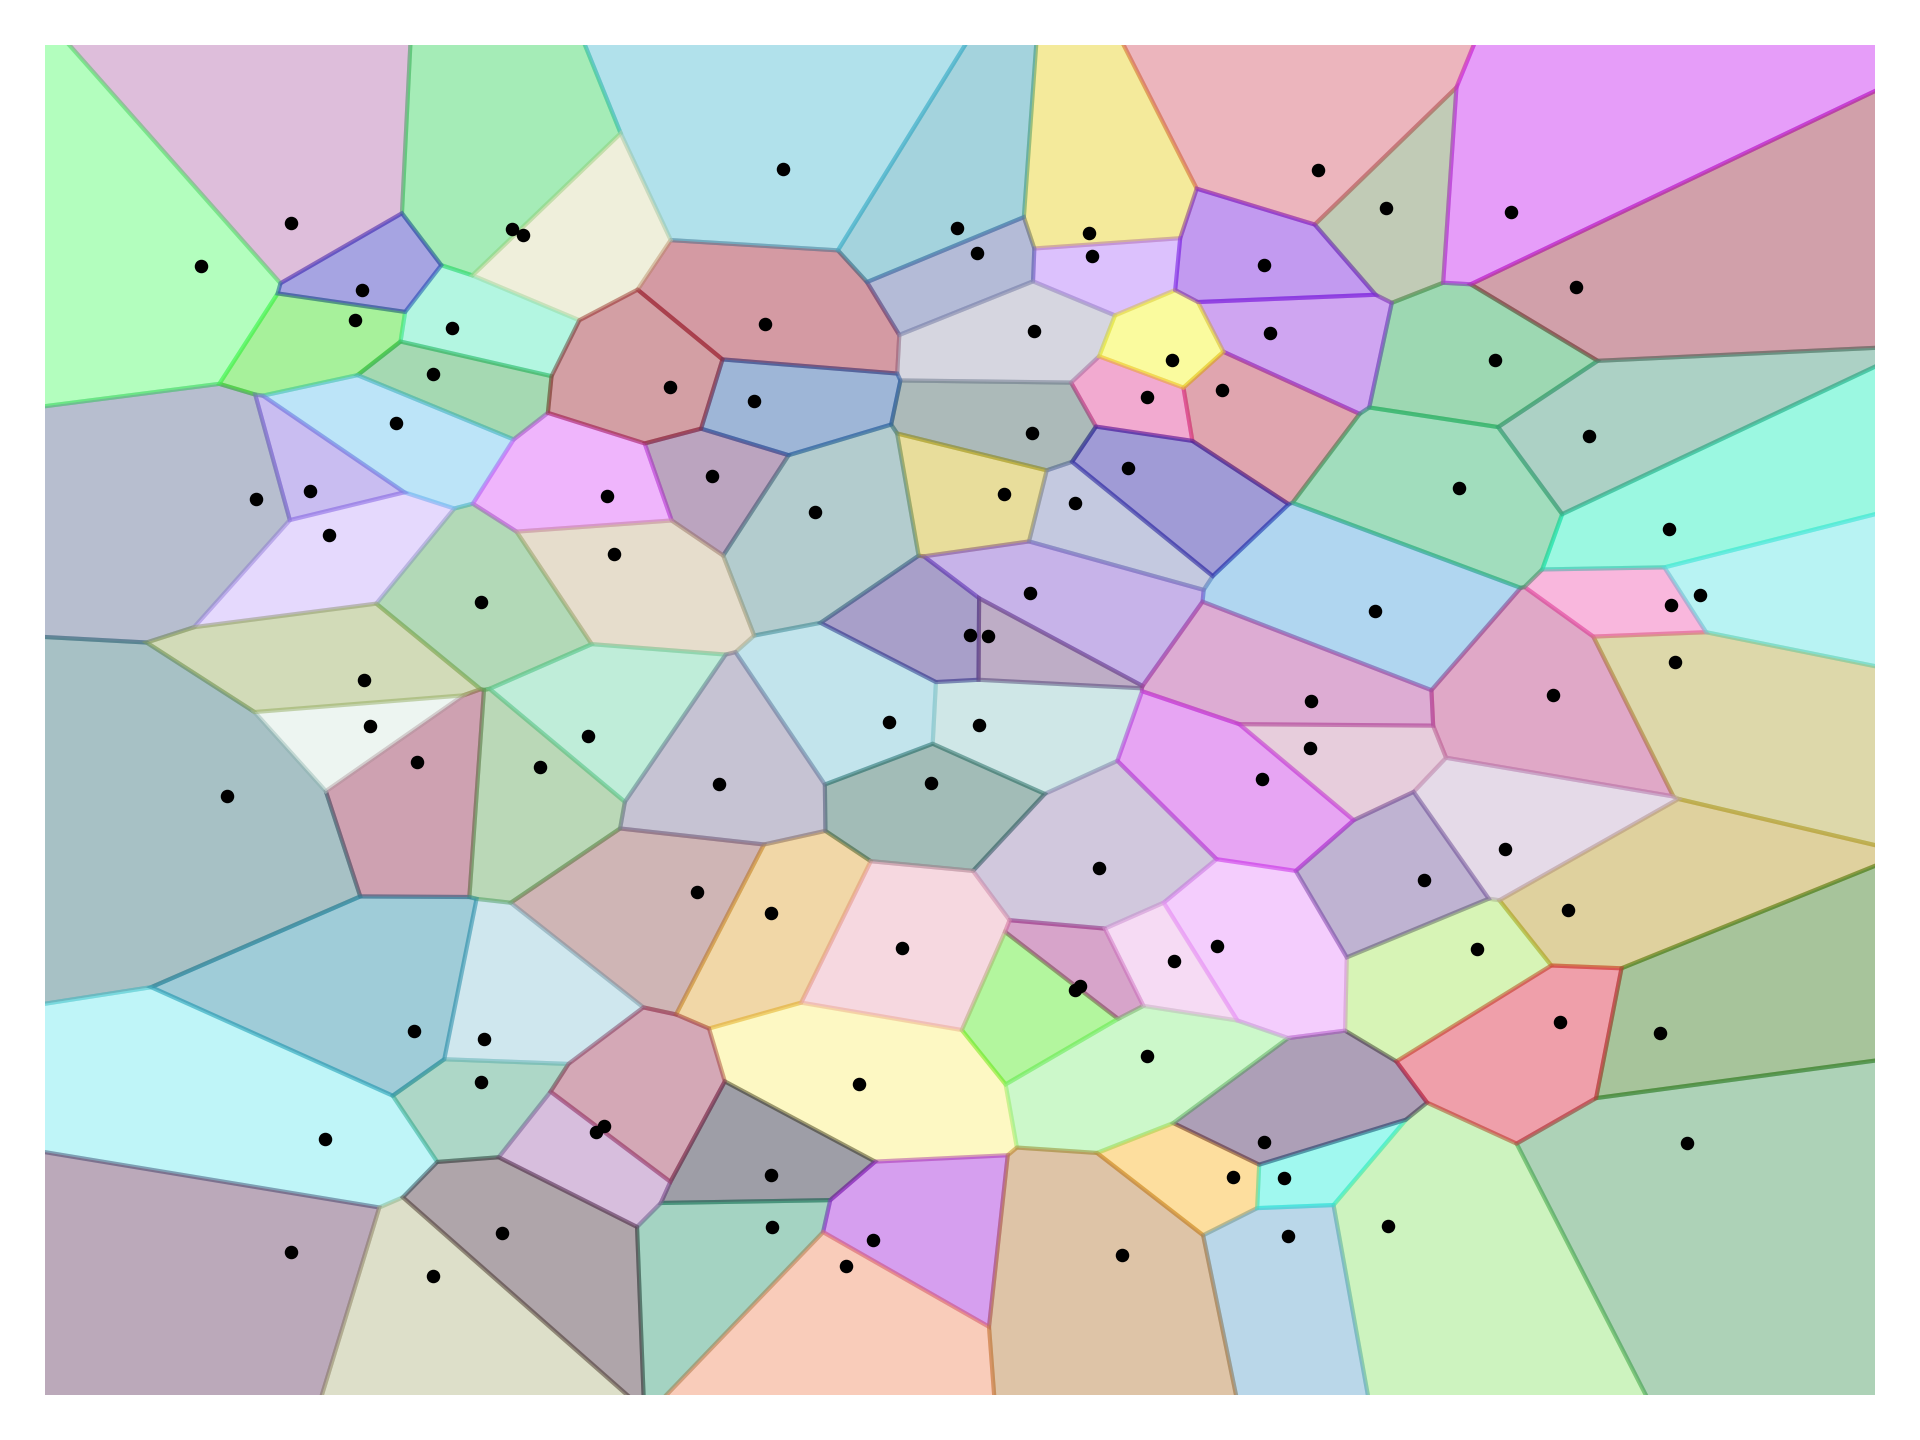
\includegraphics[scale=\myscale,scale=0.7]{figures/voronoi02b}	
\end{center}




\end{document}
